This chapter will go into the structural nature and coming together of this thesis project. The chapter starts by introducing Research through Design, as presented by Christopher Frayling and account for how this thesis has adopted the RtD approach. Then we will go into the practicalities of the project; listing and give an overview of the activities conducted. After that we will look at the project and discuss the design process up against \autocite{zimmerman_research_2014}'s five steps to carry out an RTD project. Finally, the chapter is rounded off by discussing how knowledge has been generated through analysis of installation designs and showcasing how the research question has evolved throughout the project based on theoretical and analytical findings.

\section{Research through Design}
This thesis follows an approach to research practise called Research through Design (RtD). This research approach was first coined by \autocite{frayling_1994}, in a highly influential paper where he addressed the debate and confusion at the time around what research \emph{is}, what it \emph{involves}, and what it \emph{delivers}. Frayling critiques the stereotypically perceived difference between the Research field and the Art and Design field - whereas 'researching' (stereotypically) is seen as a cognitive practice, while art and design are seen as an expressive practice \autocite[p. 5]{frayling_1994}. Concluding that since many of the motivations and practices of the two fields are alike, there is a more productive distinction in the relations between research, art, and design \autocite[p. 5]{frayling_1994}, namely: research \emph{into} art and design, research \emph{through} art and design, and research \emph{for} art and design.

According to Frayling, Research \emph{into} art and design is concerned with historical research, aesthetic and perceptual research, and research into theoretical perspectives on art and design \autocite[p. 5]{frayling_1994}. Research \emph{for} art and design, on the other hand, is research "where the end product is an artefact - where the thinking is, so to speak, \emph{embodied in the artefact}, where the goal is not communicable knowledge in the sense of verbal communication, but in the sense of visual or iconic or imagistic communication"\autocite[p. 5]{frayling_1994}. Lastly, Research \emph{through} art and design is concerned with either/ or materials research, development work (i.e., customizing a piece of technology to do something no one had considered before, and communicating the results), as well as action research (i.e., where a research diary tells, in a step-by-step way, of the experiment and result), underlining how "both the diary and the report are there to \emph{communicate the results}, which is what separates \emph{research} from the gathering of reference materials" \autocite[p. 5]{frayling_1994}.

% The way this thesis has adopted the RtD approach is perhaps a bit atypical. With the original thesis outline it was no doubt that RtD was a fitting methodology, however, eventually it became clear that it would give more data to go out and visit, collect, other installations - rather than designing my own.

% Tenker jo en liten overgang her hadde vært fint. Si NOE som helst om hvordan RtD har blitt "fulgt" gjennom prosjektet.

\section{Joint forces with two research buddies}
This thesis is based on extensive fieldwork and design activities that have been made possible because of a joint effort with two other master's students, Janni Rasmussen and Anh Thy Sandra Nguyen. In this thesis, they are referred to as research buddies. We all chose the same thesis outline but wrote separately and have developed different research agendas. In the early stages, we worked together to get to know the domain and context, for the most part discussing and sharing literature insights. Already, during spring 2021, we started to single out different areas of interest. Regardless of that, we have conducted almost all fieldwork together, yet with separate data-gathering guides and analyses.

\begin{figure}[H]
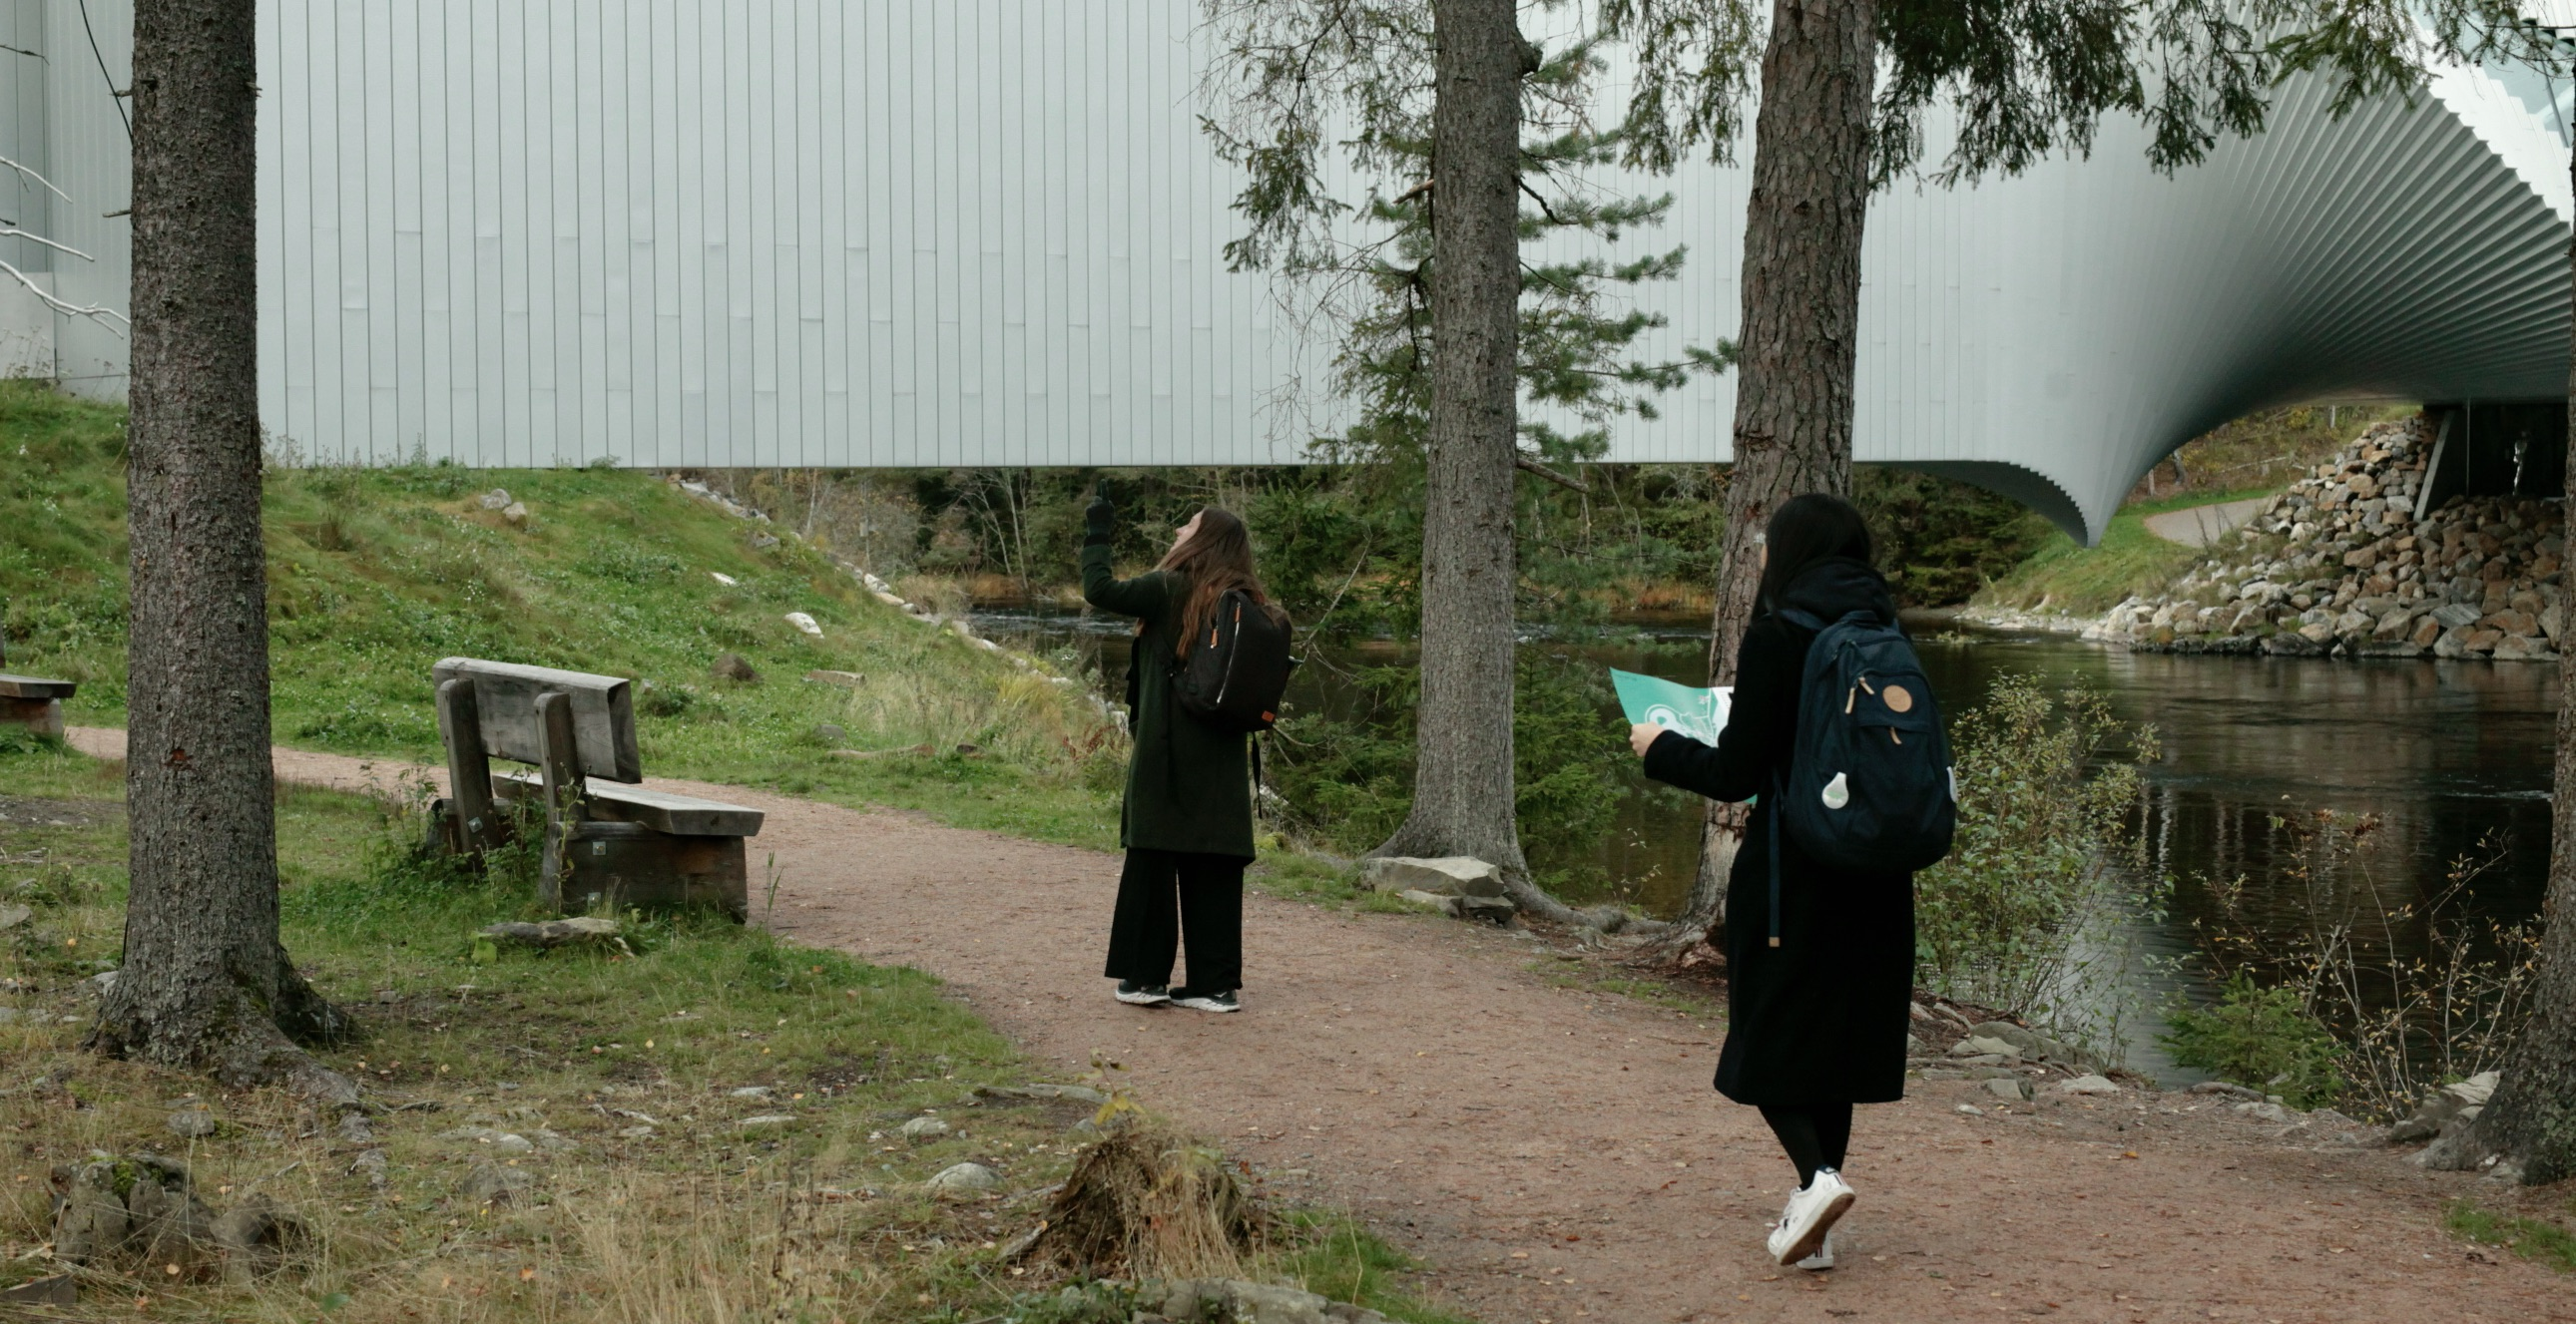
\includegraphics[width=12cm]{pictures/methodology/buddies.JPG}
\caption{The research buddies}
\centering 
\end{figure}

Janni is writing about engaging experiences with interactive installations in museums and exhibition spaces and how engagement can be facilitated with Tangible Interaction. In Sandra's study, she looks into how visitor engagement can be increased through narrative exhibitions and proposes principles for creating engaging, interactive installations in exhibition spaces.


\section{Collaborating with Klimahuset}
The original thesis outline was angled in a more practical manner; \emph{designing interactive and visual installations addressing sustainability}, and called for a partnership with a museum addressing sustainability issues. Klimahuset is one of the University of Oslo's Natural History Museums. The museum is located in the Botanical Garden at Tøyen, Oslo, newly opened in 2019. Klimahuset represents the type of space where discourses on sustainability matters can be available to citizens as a museum. The museum aim to be open and accessible to all age groups, but they have particularly aimed to engage young boys aged 14-16. Through the university partnership, Klimahuset have provided access to museum staff, Docents, and visitors and an auditorium suited for exhibitions or workshops throughout the thesis project. Klimahuset has proven to be suitable for investigating the climate crisis as an example of a museum's agenda and discourse. This provides the opportunity to investigate exhibition practise related to sustainability issues such as disseminating knowledge on Earth’s climate systems, consequences of global warming, climate crisis solutions, and what actions individuals can do to contribute to a sustainable transition and future.

\begin{figure}[H]
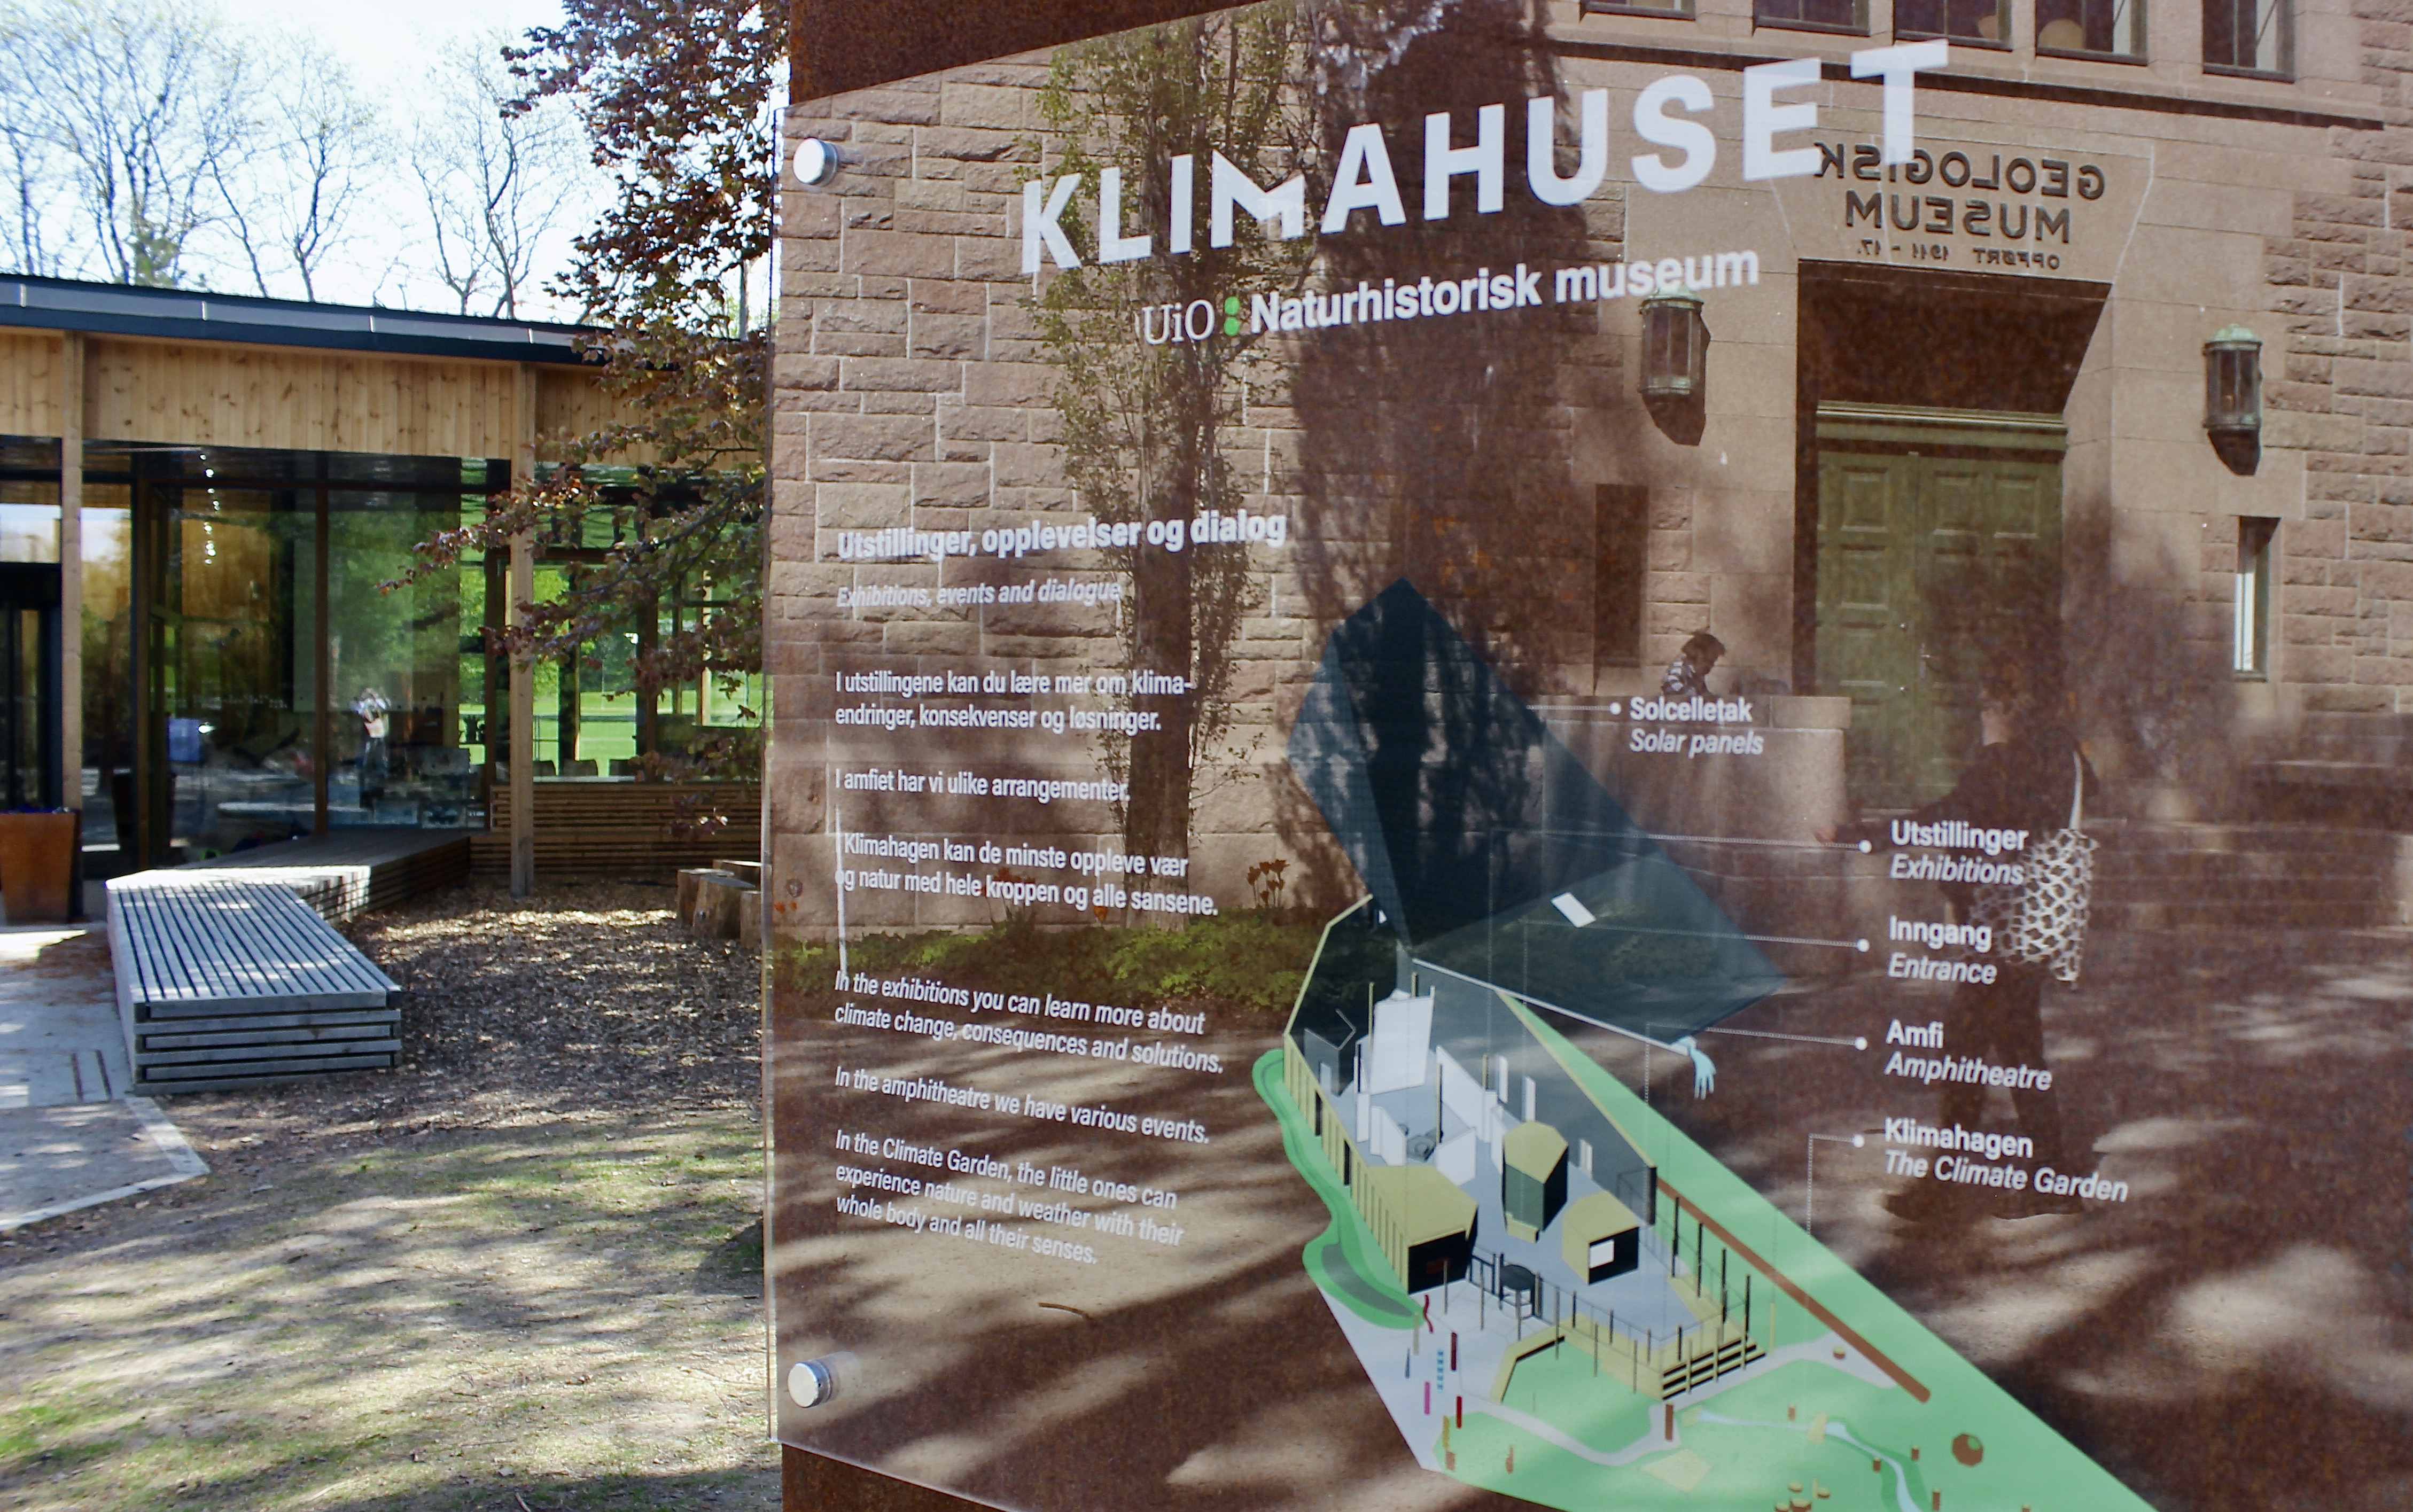
\includegraphics[width=12cm]{pictures/klimahuset/klimahuset_info.JPG}
\caption{Klimahuset entrance area}
\centering 
\end{figure}

\section{Timeline of events}
This section will account for the project timeline, presenting an overview and listing all the events that make up the project, see Figure 5.3. Together with the research buddies, we conducted all the fieldwork together. Details on each event will be provided in Chapter 6: Design Process.

\begin{figure}[H]
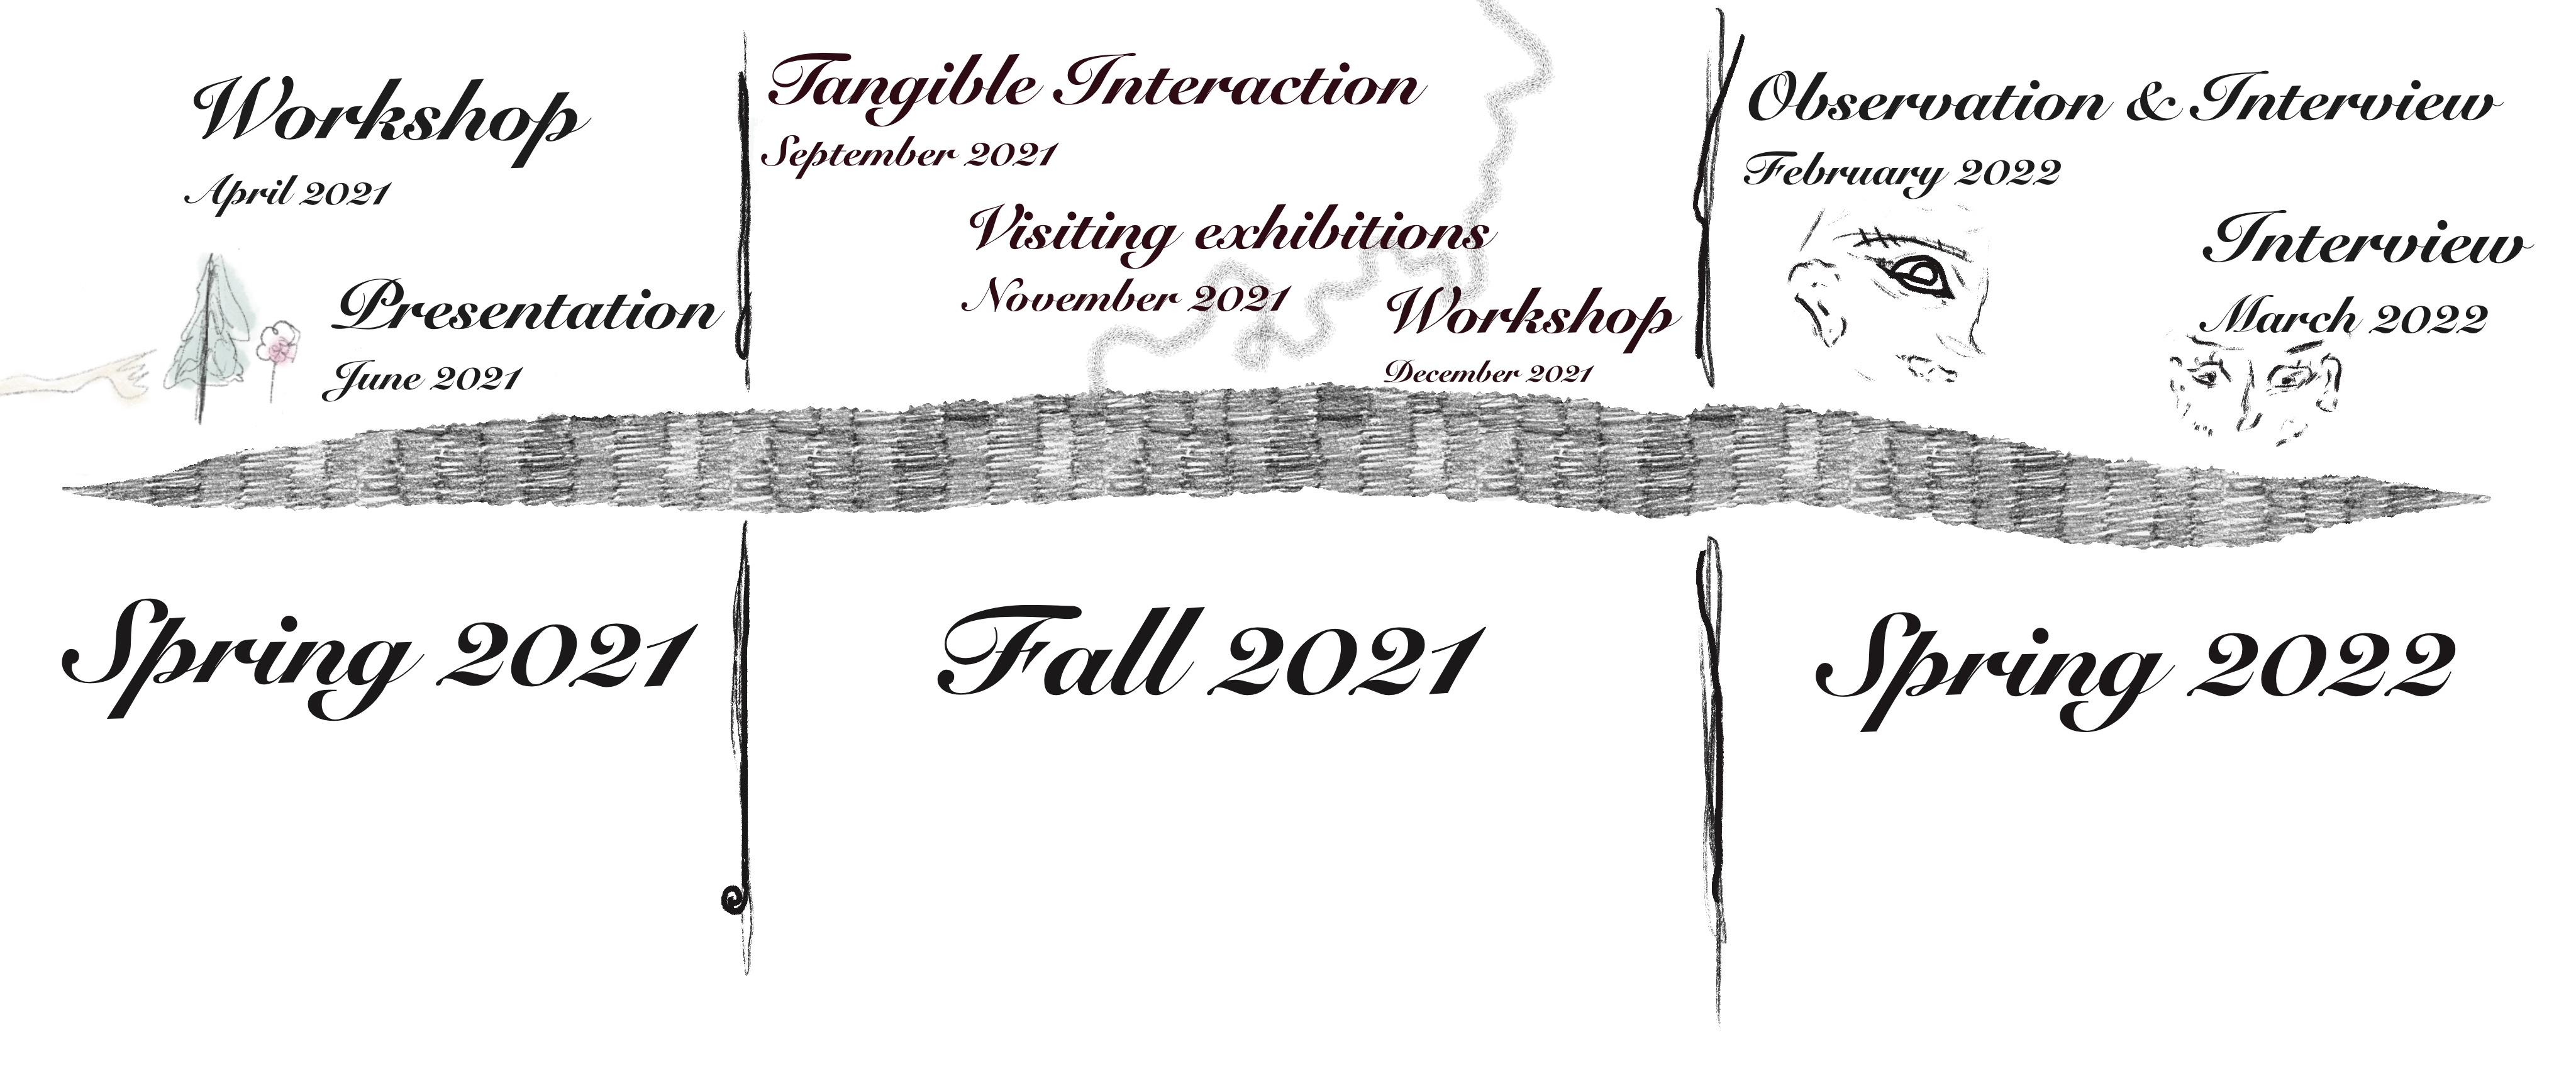
\includegraphics[width=14cm]{pictures/methodology/timeline.jpg}
\caption{Timeline of fieldwork}
\centering 
\end{figure}

The thesis project has lasted over the course of three semesters. From January to June spring of 2021, both theoretical and practical work was conducted. The original thesis outline was; \emph{designing interactive and visual installations addressing sustainability}, which called for preparation and planning for conducting a practical type of research process involving the designing of an interactive artefact. In January, we met our contact from Klimahuset and had our first viewing and walk-through of the museum's exhibition. Some weeks later, we were asked to host a workshop of our choosing that would take place in April. In February, we started a literature review focused on getting to know the museum domain and did so by reading critical literature on: exhibition practice \autocite{Thi_book}, narrative theories and learning in contemporary art museums \autocite{narrative_sitzia}, and on the subject of cultural analysis in museums \autocite{Miekebal_book}, as is evident in Chapter 2: Modern Museums and sustainability. To explore the sustainability aspects of the current RQ (\emph{designing interactive and visual installations addressing sustainability}), I worked conceptually and explored the topic; a distanced relationship to nature. This later manifested itself in the low-fidelity prototype that was presented at Klimahuset in June 2021; see section 6.3 in Chapter 6: Design Process.

All this work contributed to narrowing down the research area of interest and formulating a new research question; \textit{How can one design for meaningful interactive experiences in a museum space addressing sustainability?}.

Next semester, August to December fall 2021, is where most practical research efforts were done. In September, we participated in a course about Tangible Interaction. Through this course, we were put in small teams who conceptualized, designed, and exhibited an interactive installation during the course duration of one month. This resulted in three installations that have been used in analysis, see section 6.4 in Chapter 6: Design Process. Then came November, and we decided to visit different museums that exhibited interactive installations to experience, observe and collect data on different installations. The museums and exhibitions we visited is accounted for in sections 6.5, 6.6, 6.7, and 6.10 in Chapter 6: Design process. In late December 2021, the Tangible Interaction group I was a part of was requested to exhibit our installation for a group of first-year master's students interested in writing about energy visualization, see section 6.8 in Chapter 6: Design Process. Then comes Spring 2022, where the main focus is writing up the thesis. In February, we were given the opportunity to observe two school classes in Klimahuset and given a little time to interview the working Docents - which we accepted. This is accounted for in section 6.9, Chapter 6: Design Process. In March, our supervisor reached out to the newly opened MUNCH museum and presented us with the opportunity to interview a concept developer working there. % Accounted for in??....

\begin{table}[h]
\centering
\begin{tabular}{| l | l|}
\hline
\textbf{Month} & \textbf{Event}\\
\hline
Jan. 21 & Initial contact and visiting Klimahuset for the first time \\
Feb. 21 & Started literature review on museums \\
Apr. 21 & Hosted a workshop for members of staff from Klimahuset \\
May 21 & Prototyped low-fid installation exploring input through plants \\
Jun. 21 & Held a presentation w/ RB.* at Klimahuset \\
Sep. 21 & Tangible Interaction course: designed an installation \\
Nov. 21 & Visited 5 interactive exhibitions \\
Dec. 21 & Held an energy visualisation workshop with Qi-installation \\
Feb. 22 & Observation of two school children classes in Klimahuset \\
Feb. 22 & Interview with two of Klimahuset's Docents \\
Mar. 22 & Interview w/ concept developer at Munch Museum \\
Apr. 22 & Analysis workshop sessions \\
May 22 & Visited one more interactive exhibition \\
\hline
\end{tabular}
\caption{Detailed table of fieldwork events}{RB= research buddies}
\end{table}

\section{How the thesis have developed over time}
To describe and make clear how the thesis have developed over time, I will use \autocite{zimmerman_research_2014} model for interaction designers to carry out an RtD research project. "An RtD project gets documented such that other researchers can reproduce the process; however, there is no expectation that others following the same process would produce the same or even a similar final artifact" \autocite[p. 168]{zimmerman_research_2014}. To carry out an RtD research project, Zimmerman \& Forlizzi propose a team to follow five steps:

\begin{itemize}
    \item 1. Select
    \item 2. Design
    \item 3. Evaluate
    \item 4. Reflect and Disseminate
    \item 5. Repeat
\end{itemize}

This is how this thesis project fits into Zimmerman's five steps/ phases, and have developed over time:

\subsection{Step 1: Select}
\textit{Select} involves choosing a research problem or design opportunity worthy of investigation and considering whether the research problem lends itself to investigation via RtD \autocite[p. 185]{zimmerman_research_2014}. This project started with the original outline to \emph{designing visual and interactive installations addressing sustainability}. The thesis called for students interested in designing interactive and visual installations who wanted to explore how one could use installations to engage citizens in discourses. This set the first constraints in the research project design, knowing for one, that there was to be made an installation of some sort during the project, and two, therefore, the methodological approach would involve design activities and prototyping. However, the broadness of the thesis outline called for decisions on what \textit{sustainability} should encompass or represent in terms of the research scope and design. The same goes for the role of the \textit{exhibition space}, and \textit{interactivity}.

To inform the decision process, I started a literature review meant to ground the inquiries on both the museum domain and the HCI community concerned with museum exhibition and experience design as a way to get to know the design context from a theoretical point-of-view. The literature review was coordinated with the research buddies; we shared literature insights and had regular discussions on the topics we read. Table 5.2 showcases the inquiries that have guided the literature review. The literature review has been a "living" work-in-progress throughout the thesis project duration. It is accounted for and summed up in chapters 2 and 3. In Chapter 2, the chapter's structure aim to reflect how the literature review has been used as a theoretically grounded vocabulary and lens during fieldwork and design efforts. Moreover, the literature review has been crucial in selecting a design opportunity and research context, in line with Zimmerman's \emph{select} step.

\begin{table}[H]
\centering
\begin{tabular}{| l |}
\hline
\textbf{Inquiry} \\
\hline
Museology practise \\
Narrative theories and learning in contemporary art museums \\
Dissemination: from knowledge to narrative \\
Museum exhibition design in HCI \\
Design for sustainability and the Anthropocene \\
Augmenting exhibition design through the use of technology \\
Understanding and supporting the museum experience \\
Design as meaning making \\
\hline
\end{tabular}
\caption{Literature review inquiries}
\end{table}

\break
"Selecting is an iterative process of trying many different things until the team agrees" \autocite[p. 185]{zimmerman_research_2014}. Based on and inspired by literature review readings, it became clear quite early that I wanted the design opportunity to reflect a place-centred approach to the research context. See Figure 5.4 for a visualization of the design opportunity and research context. The way I saw it, I wanted the \textit{sustainability} term from the original outline to simply represent a contemporary discourse. Therefore, it was decided that in the scope of this thesis, \emph{the climate crisis} represented a contemporary issue disseminated in museums. Every museum have a discourse, either related to the whole museum like Klimahuset, or many discourses spread across several exhibitions like MUNCH. That is why \emph{the climate crisis: a contemporary issue}, is placed in the middle of Figure 5.4. Again, inspired by literature review readings, what more than anything characterizes the climate crisis as a discourse is that it calls for public discussion, individual reflections, and social change. What I, through literature review, later would synthesise as dialogic behaviour. In early selecting stage, I saw the design opportunity in the scope of the thesis project being; to design for holistic, meaningful experiences in a hybrid museum space. Where \emph{interactivity} would be designed to support or extend these meaningful experiences.

\begin{figure}[H]
\centering
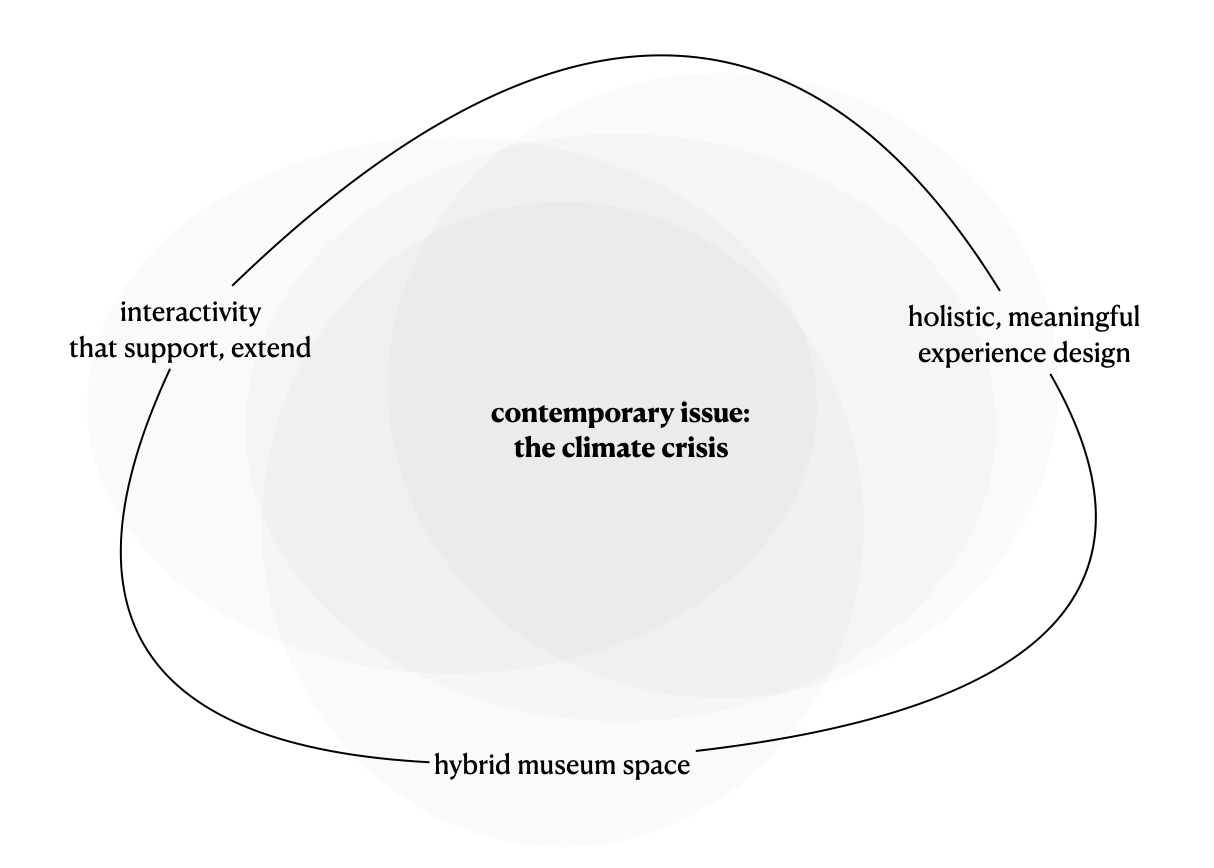
\includegraphics[width=12.5cm]{pictures/methodology/problem_sphere.png}
\caption{Design opportunity space and research context sphere}
\end{figure}

\subsection{Step 2: Design}
\textit{Design} involves the beginning of design activities, ranging from literature review to understanding the state of the art, conducting fieldwork, holding design workshops, playing with new material or exploring ideas in the studio \autocite[p. 185]{zimmerman_research_2014}. The team should also consider which RtD practise to follow (Lab, Field or Showroom), and if they wish to mix the practises together \autocite[p. 185]{zimmerman_research_2014}. Guided by the original thesis outline, I started doing design activities quite early on during the spring 2021, and parts of the fall 2021 (ref timeline of fieldwork Figure 5.3). These design activities are listed in Table 5.3. Due to the characteristics of the climate crisis as a discourse and central theme in the problem sphere, I wanted the installation design to reflect a critical, or provocative nature that would force people to think, notice, or reconsider some aspect of the world \autocite[p. 173]{zimmerman_research_2014}. Naturally, the chosen RtD practise to follow was Showroom. The literature review have been accounted for being present in the select stage as well, serving a theoretical referential role to the shaping of the design opportunity and research context. In relation to the design activities, the literature review have been formative in the shaping of \emph{the framework without a name}. The literature review conducted during the \emph{design} step, were specially concerned with designing for meaningfulness.

\begin{table}[H]
\centering
\begin{tabular}{| l | l | l |}
\hline
\textbf{Type} & \textbf{Name} & \textbf{Ref. Section:}\\
\hline
Literature review & Modern museums and sustainability & chpt. 2, 3 \\
Workshop & Narratives and storytelling & 6.2 \\
Prototyping & Exploring input through plants & 6.3 \\
Presentation & Exploring input through plants & 6.3 \\
Prototyping & Qi & 6.4.3 \\
Exhibition & Qi & 6.4.3 \\
Critiquing & Visited 7 exhibitions & 6.5-6.7, 6.10\\
Observation & Climate Dialogue w/ 2 school classes & 6.9\\
Interview & Concept Developer & \\
\hline
\end{tabular}
\caption{Design activities conducted throughout the project}
\end{table}

 An important aspect of the early stages of the \emph{Design} step, is that the team is searching to understand the state of the world; how they might offer a new perspective, or a new problem framing, which provides a path to the preferred future \autocite[p. 185]{zimmerman_research_2014}. These concerns felt already kind of answered in the shaping of the design opportunity and research context space (ref Figure 5.4). When doing design activities, the valuable insight that was gained through the practicalities of conceptualising, designing and implementing an installation, first low-fidelity with the \emph{exploring input through plants}, and then more high-fidelity with the \emph{Qi} installation, was that I began to question whether designing an installation was a good fit lended to investigate and answer the design opportunity sphere. These experiences, plus time-constraints, was the dominant factors for deciding to critique interactive installations made by others, rather than design one by myself, to ensure that we would have enough data-material to be able to evaluate and apply \emph{the framework without a name}, and answer the overarching research question. 


\subsection{Step 3: Evaluate}
Throughout the process of making and critiquing, the team should \textit{evaluate} and continually challenge their initial framing while documenting the design moves and rationale for these moves \autocite[p. 185]{zimmerman_research_2014}. During this thesis, two design-move changes in the research question have influenced the direction of the thesis project, the results, and the scientific contribution. To showcase this, I have visualized the project timeline rooted in the evolution of the research question, see Table 5.4: Research question evolution. The table is meant to be read as a linear timeline from project start to end, where the horizontal arrows represent both \emph{the passing of time} variable and a design move. The vertical axis is based upon \autocite{beck_examining_2016}'s list of core elements of a research publication, and the horizontal axis is based upon \autocite{zimmerman_research_2014}'s five steps to carry out an RtD research project. Table 5.4 aims to illustrate how the research project evolution has been shaped by design activities and their findings, and the use of theory. 

To elaborate a little on \autocite{beck_examining_2016}'s list of core elements of a research publication and why they are relevant up against \autocite{zimmerman_research_2014} - they were developed as part of Beck \& Stolterman's process of identifying models of theory use. The list of core elements of a research publication aims to represent the relationships and interactions between theory and the other core elements in the papers that were examined \autocite[p. 129]{beck_examining_2016}. I found these to be useful in visualizing the design moves and rationale for these moves \autocite{zimmerman_research_2014}. The core elements are as follows: \textit{question, examination, findings, and theory}. "Questions" identify the needs or interests that the researcher deems worthy of understanding, explaining, predicting, or describing" \autocite[p. 129]{beck_examining_2016}. In table 5.4, this column is named \textit{RQ timeline} and contains the research questions and main inquiries that have shaped the research project direction. "Examination" captures the approach taken to answer the question—that is, and includes all forms of analytical or empirical work done by the researcher to investigate the question at hand \autocite[p. 129]{beck_examining_2016}. In table 5.4, this column is named \textit{Examination} and contains the design activities related to the research question or inquiry. These design activities are the same that we have just accounted for in Step 2: Design. "Findings" refer to the outcome of this examination \autocite[p. 129]{beck_examining_2016}, and is named correspondingly. "Theory" is the fourth core element in the models, referring to theory's role and use throughout the project - which has been accounted for in Chapter 4, section 4.1. I found that setting \autocite{zimmerman_research_2014} and \autocite{beck_examining_2016} up against each other this way, provided a quite detailed and explicit depiction of the design moves and capturing the main reasons for these framing changes. While also serving as a sort of methodological timeline of the thesis project evolution as well.

\begin{table}[H]
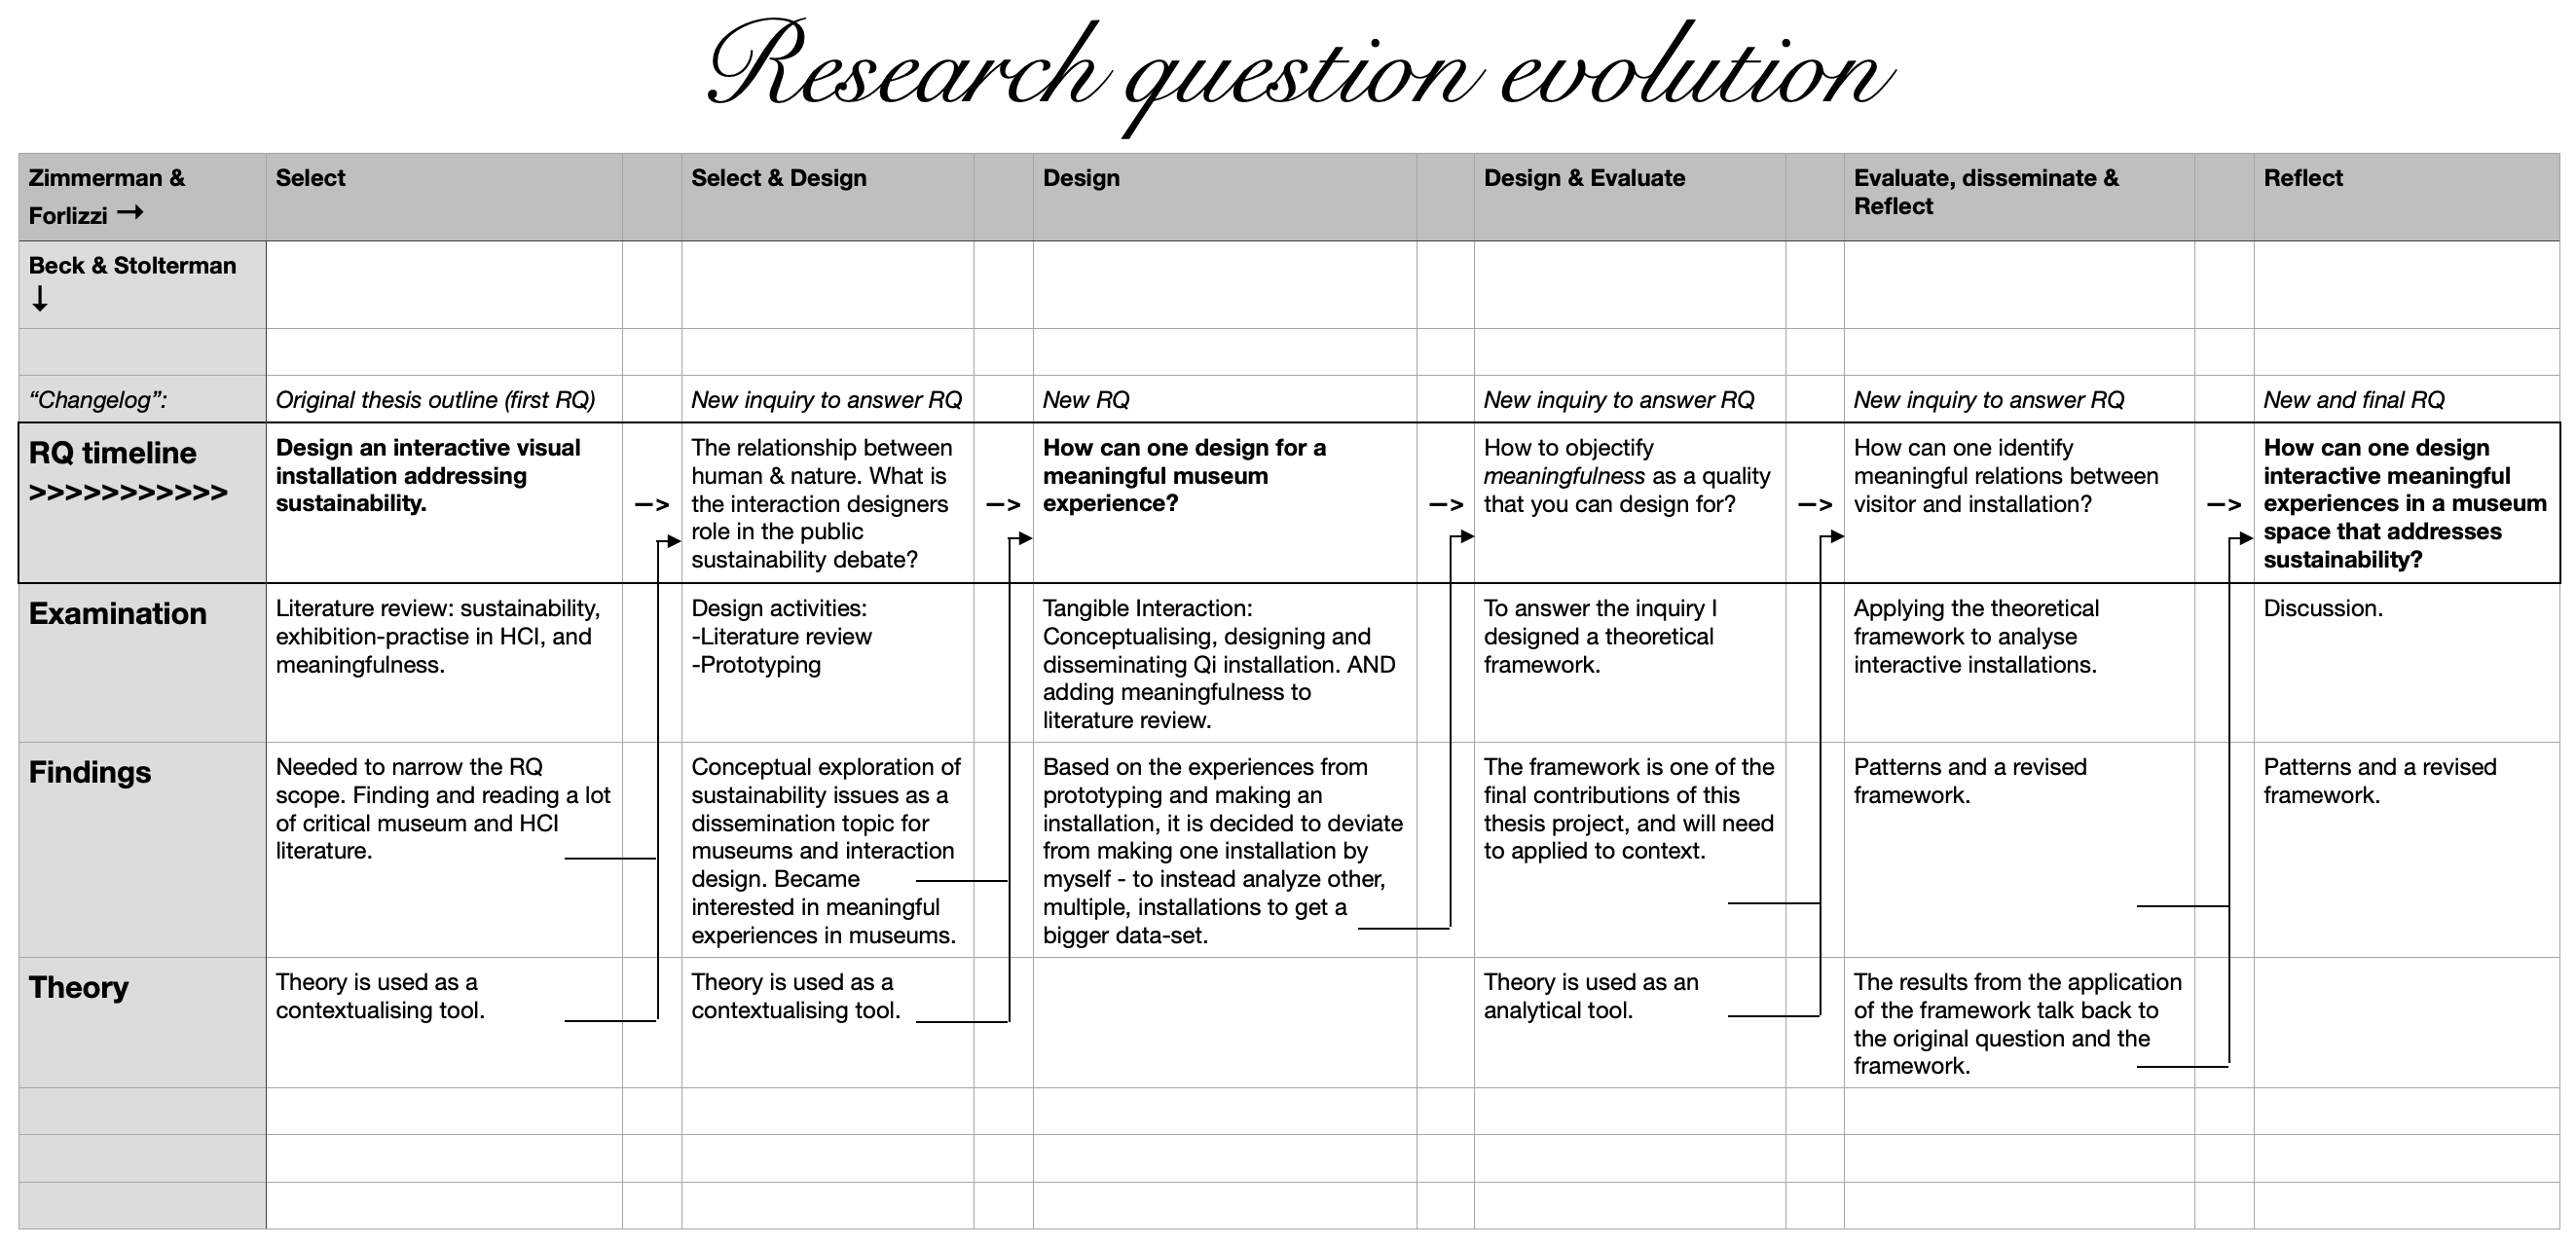
\includegraphics[width=22cm, angle=90]{pictures/methodology/rq_evolution.png}
\caption{Research question evolution}
\centering
\end{table}

"When the team has an artifact they like, they should evaluate it based on the concerns of the specific RtD practice they selected (Lab, Field, or Showroom) and on concerns specific to their research question" \autocite[p. 186]{zimmerman_research_2014}. "Work following the Showroom practice will likely involve the installation of a working system in a gallery or in some other place where people outside of the research team can experience the design and can begin to question the world around them" \autocite[p. 186]{zimmerman_research_2014}. Based on the experiences from prototyping and making an installation during fall 2021, halfway through the project it was decided to deviate from making one installation by myself - to instead analyze other, multiple, installations to get a bigger data-set. Before we embark further to Step 4: Reflect \& Disseminate, I want to shortly account for how this new design-move change still lends the new research question and scope to investigation via RtD practise. The main intention of analysing existing interactive installations rather than designing, implementing, and evaluating one installation, has been to help inform the overarching research question. I wanted to complement my theoretically informed framework with knowledge from analyzing and critiquing installation designs, to use the strengths of both theory and design to synthesise a solid framework. Along these lines, Bardzell et.al argue that while the \emph{intentions} of the object's designer are important and annotations are a good mechanism to articulate them, the critical reception of objects can be equally generative of RtD's knowledge impacts \autocite[p. 2093]{bardzell_immodest_2015}. This support the notion of why it made sense to rather make use of, and critiquing, other installation designs - because they can serve an equally generative knowledge production in comparison with simply critiquing one. At this point, the knowledge obtained related to the research context and design opportunity sphere, strengthened the confidence of being able to do a theoretically grounded and just critiquing. Which I considered a better way to apply the theoretical framework and in that sense generate more knowledge than designing.


\subsection{Step 4: Reflect \& Disseminate}
"Following the evaluations, the team should reflect on what they have learned and then work to disseminate the research. Dissemination can happen in terms of publication in peer-reviewed venues such as conferences or journals. It might also take the form of a video or demonstration." \autocite[p. 186]{zimmerman_research_2014}. In this thesis, the reflect and disseminate step are accounted for and documented throughout Chapter 7: Analysis, where the framework has been applied and the creation of patterns. The structure of chapter 2 and 3 aim to reflect and disseminate domain knowledge through the Oxford-dictionary composition of different terms and concepts. 

\subsection{Step 5: Repeat}
"The final step in the process is to repeat. \autocite{koskinen_2013} note that RtD researchers who produce the best research results do so by repeatedly investigating the same situation. It is through the development of research programs much more than through individual projects that the best results emerge" \autocite[p. 186]{zimmerman_research_2014}. In terms of the thesis project duration and scope, this thesis project has not been able to do or facilitate for repeating steps. That would have to be considered Future Work. One way of exploring what this Future Work would encompass, could be through  \autocite{fallman_triangle_2008}'s interaction design research triangle of Design Practise, Design Study and Design Exploration. See Figure 5.5 for: the model in its most basic form: 

\begin{figure}[H]
\centering
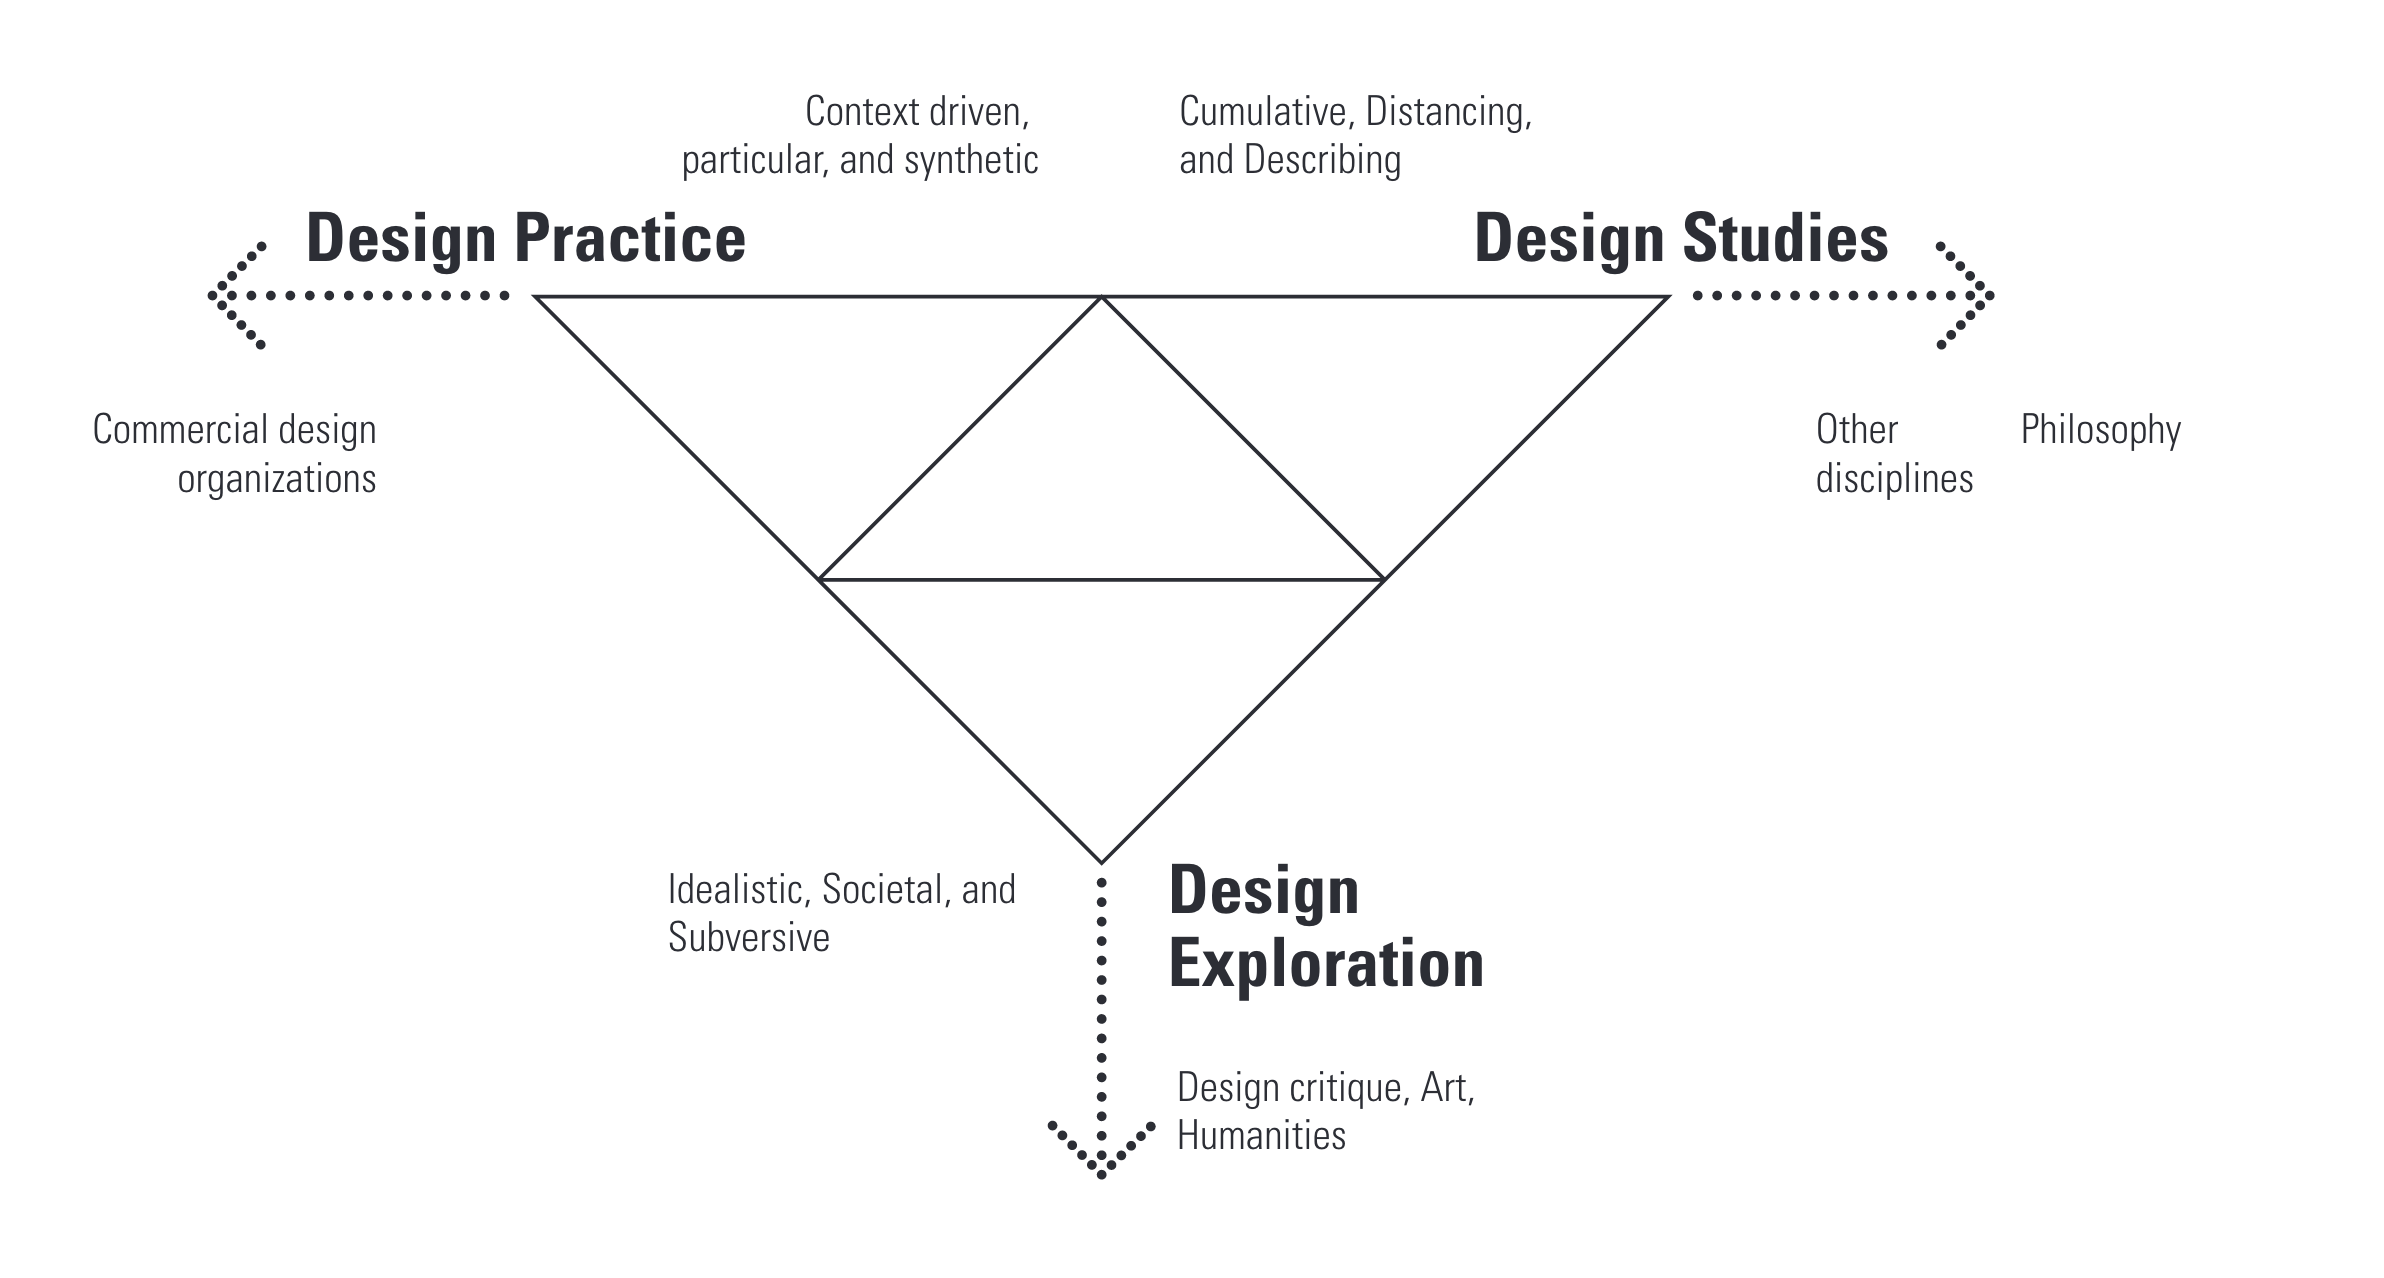
\includegraphics[width=12.5cm]{pictures/methodology/fallman_triangle.png}
\caption{The model of interaction design research in its most basic form.}
\autocite[p. 5]{fallman_triangle_2008}
\end{figure}

As a design discipline, interaction design’s core can be found in an orientation towards the shaping of digital artefact, products, services, and spaces - with particular attention paid to the qualities of the user experience \autocite[p. 4]{fallman_triangle_2008}. In Fallman’s use of the model, the most interesting and rewarding results in interaction design research come not from taking a specific position in the model, but rather from moving or drifting in between different positions in the triangle model. As visualized in Figure 5.6 - this thesis has positioned itself and moved between Design Studies and Design Exploration through a thorough literature review, prototyping, and critiquing of interactive installations: 

 \begin{figure}[H]
\centering
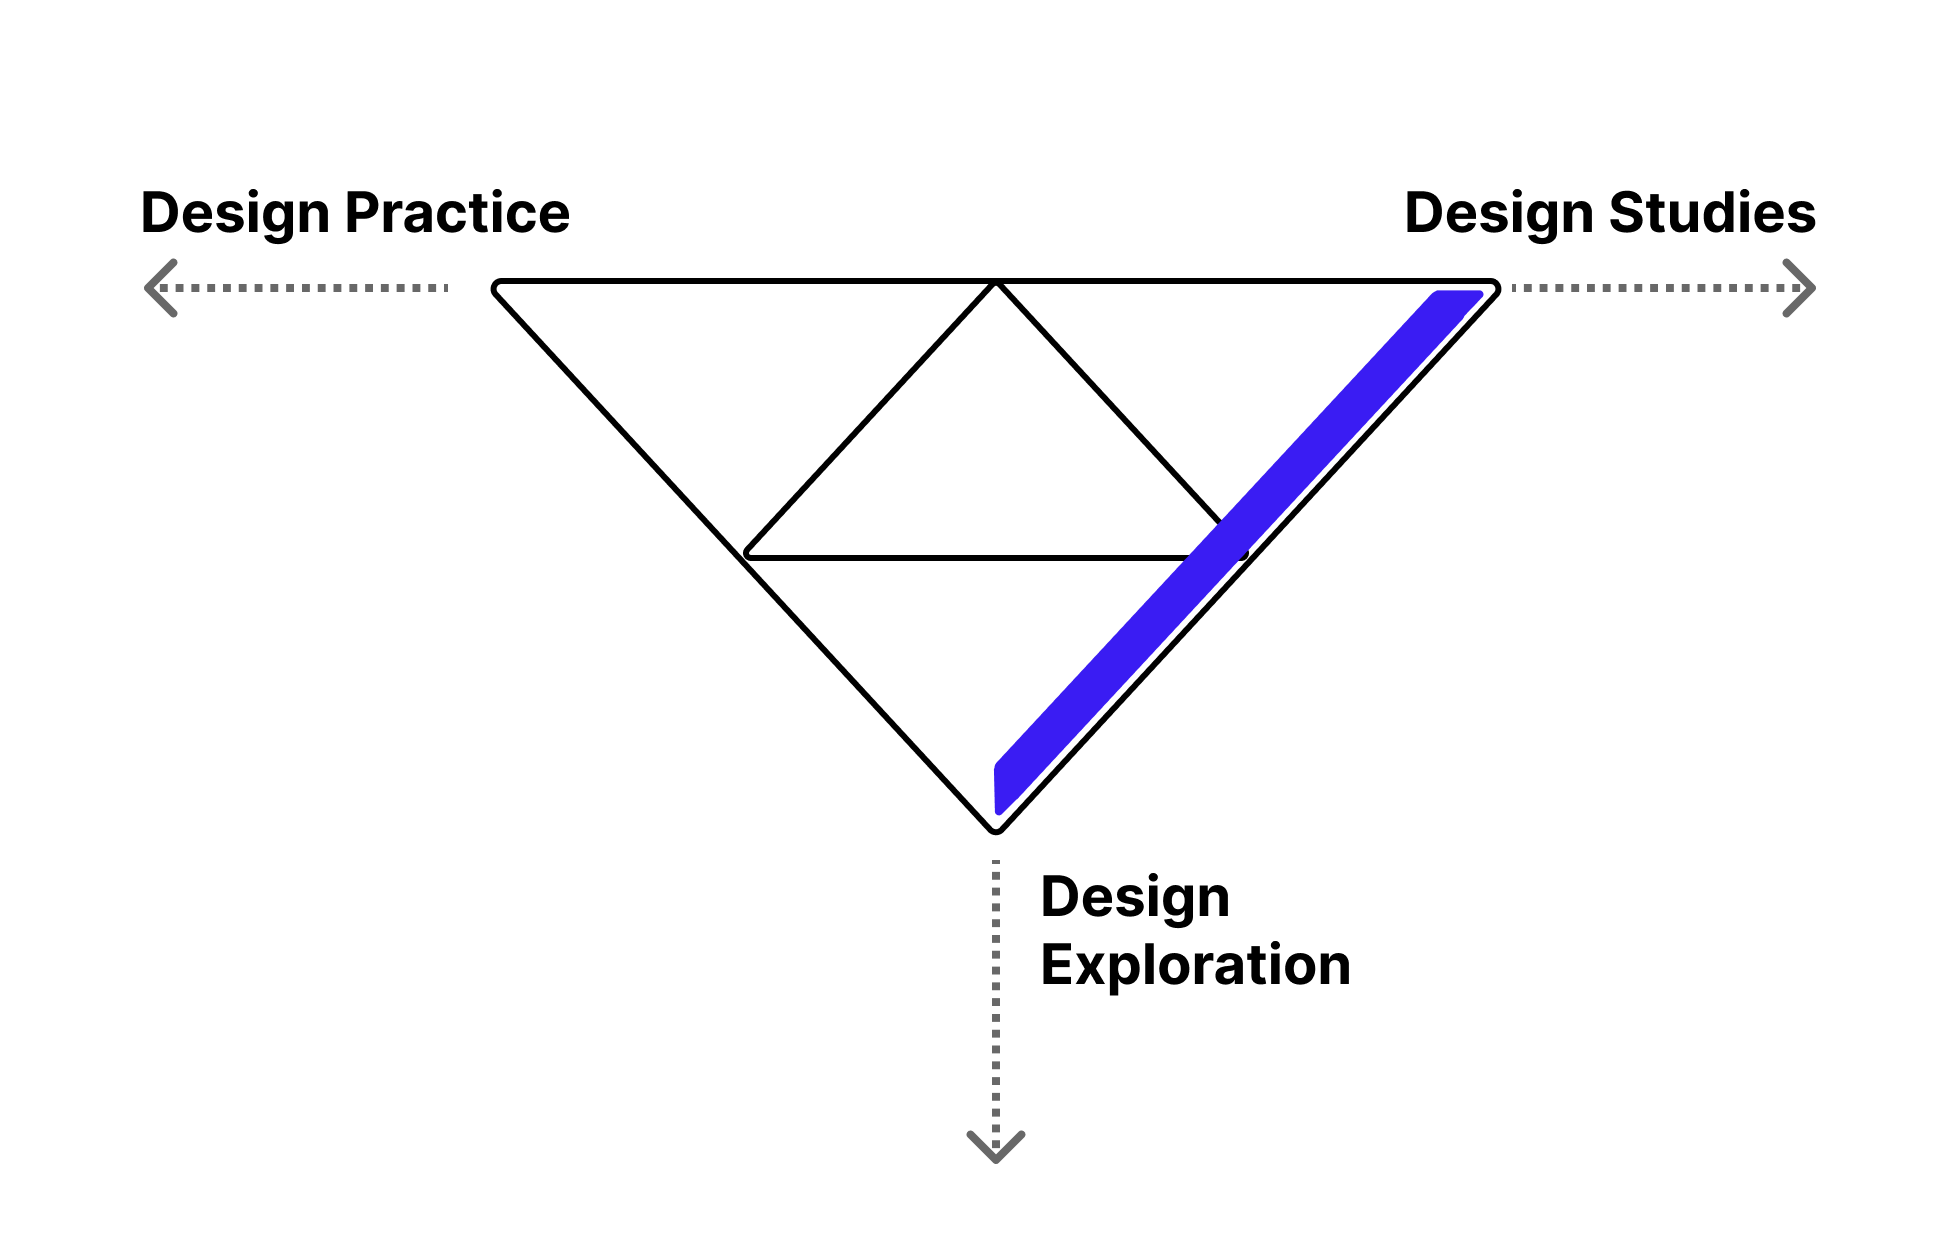
\includegraphics[width=10cm]{pictures/methodology/fallman_applied.png}
\caption{Moving between Design Study and Design Exploration}
\end{figure}

Future work would encompass drifting from Design Practise to either Design Study or Design Exploration, as visualized in Figure 5.7. Involving stakeholders, museum and design practitioners, and of course review and collect more comprehensive visitor accounts of experiences would prove fruitful as a repeating investigation of this design opportunity space and research context.

\begin{figure}[H]
\centering
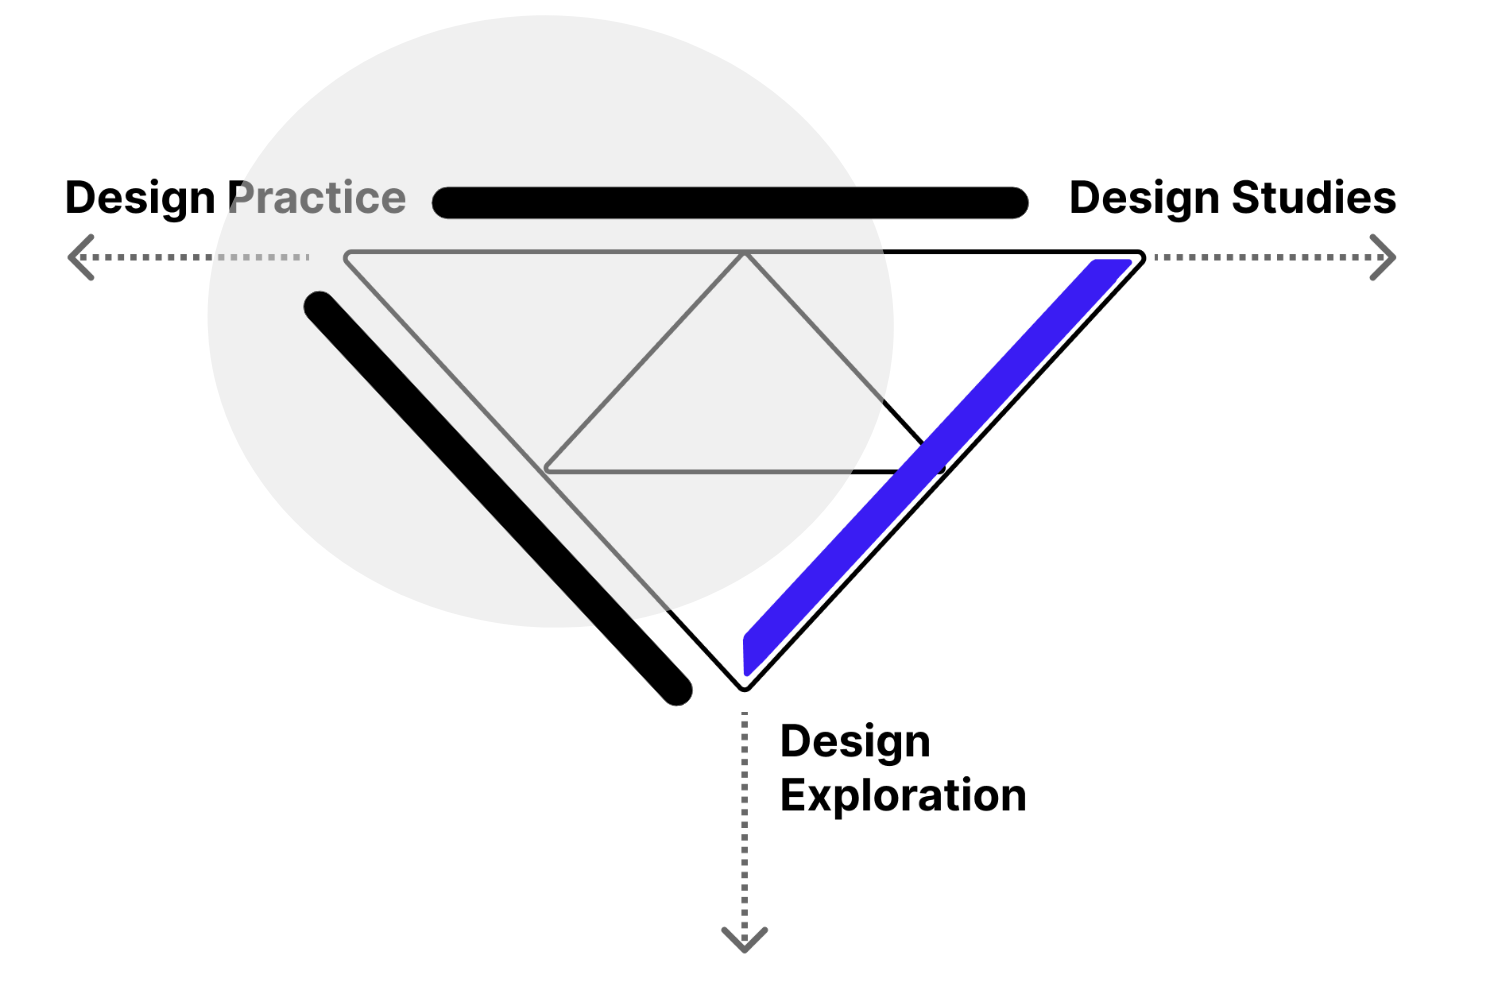
\includegraphics[width=10cm]{pictures/methodology/fallman_future.png}
\caption{Future work movements in this research context}
\end{figure}
    